\documentclass[tikz,border=2]{standalone}
\newcommand{\leadblock}{C^{\mathrm{lead}}}
\newcommand{\trailblock}{C^{\mathrm{trail}}}
\usetikzlibrary{decorations.pathreplacing,shadows,arrows,shapes,positioning,calc,backgrounds,fit}
% Define the layers to draw the diagram
%
\begin{document}
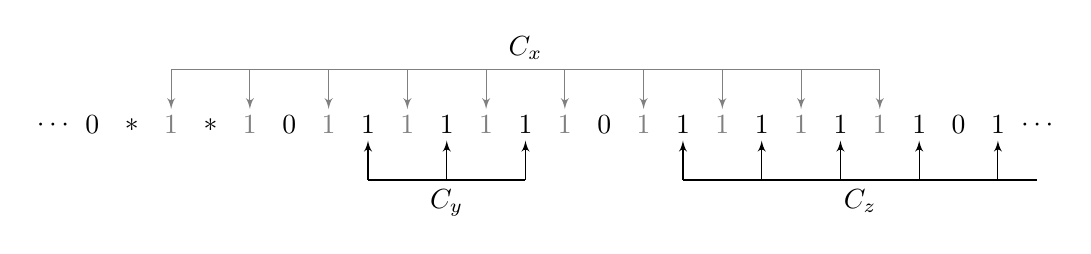
\begin{tikzpicture}
[node distance=1cm,
block/.style={thick},
vertex/.style={shape=circle,draw=black,inner sep=2pt},
dedge/.style={>=latex', shorten >=.0pt, shorten <=.0pt},
myedge/.style={thick}]

% large block Cx
\draw (-.5,0) node {$\cdots$};
\draw (0,0) node {$0$};
\draw (0.5,0) node {$*$};
\foreach \x in {1,...,10}
\draw[dedge,<-,gray] (\x,0) node {$1$}+(0,.2) -- (\x,.7) ;
\draw (11,0) node {$0$};

\draw (1.5,0) node {$*$};
\draw[gray] (1,.7) -- (10,.7) node[midway,above,black] {$C_x$};

% contained block Cy
\draw (2.5,0) node {$0$};
\foreach \x in {3.5,4.5,5.5}
\draw[dedge,<-] (\x,0) node {$1$}+(0,-.2) -- (\x,-.7) ;
\draw (6.5,0) node {$0$};
\draw (3.5,-.7) -- (5.5,-.7) node[midway,below,black] {$C_y$};

% intersecting block Cz
\foreach \x in {7.5,8.5,...,11.5}
\draw[dedge,<-] (\x,0) node {$1$}+(0,-.2) -- (\x,-.7) ;
\draw (12,0) node {$\cdots$};
\draw (7.5,-.7) -- (12,-.7) node[midway,below,black] {$C_z$};

% band boundaries
%\draw[dashed] (2,-2) -- (2,2) node[midway,left] {\large $B_{m-1}$};
%\draw[dashed] (4,-2) -- (4,2); % node[midway,left] {$B_{m-1}$};
%\draw[dashed] (10,-2) -- (10,2); % node[left] {\Large $B_{m}$};
%\draw[dashed] (12,-2) -- (12,2) node[midway,right] {\large $B_{m+1}$};
%\node at (3,0) {$\cdots 00\cdots$};
%\node at (11,0) {$\cdots 00\cdots$};
%
%% D_B
%\draw[block,|-|] (4,.5) -- (6,.5) node[midway,below] (c1) {$C'_1$};
%\node[left,above] (lead) at (3,1) {$\leadblock(B_m)$};
%\draw[dedge,->] (lead) -- ($(c1)+(0,.4)$);
%\draw[block,|-|] (5.5,0) -- (8.5,0) node[midway,below] (c2) {$C'_2$};
%\draw[block,|-|] (8,-.5) -- (10,-.5) node[midway,below] (c3) {$C'_3$};
%\node[right,below] (trail) at (11,-1) {$\trailblock(B_m)$};
%\draw[dedge,->] (trail) -- ($(c3)+(.25,0.2)$);
%\node (DB) at (5,-1.5) {$D_{B_m}$};
%\draw[dedge,->] (c1) -- (DB);
%\draw[dedge,->] (c2) -- (DB);
%\draw[dedge,->] (c3) -- (DB);
%
%\draw [decorate,decoration={brace,amplitude=10pt,mirror,raise=4pt},yshift=0pt]
%(4,-2) -- (10,-2) node [midway,below,yshift=-.5cm] {\Large $B_m$};
%
%% properly contained blocks
%\draw[block,|-|] (4.5,1) -- (5,1) node[midway,above] (p1) {};
%\draw[block,|-|] (6.25,.5) -- (6.75,.5) node[midway,above] (p2) {};
%\draw[block,|-|] (7,.5) -- (7.5,.5) node[midway,above] (p3) {};
%\node (prop) at (6.25,1.75) {\small Properly contained blocks};
%\draw[dedge,<-] (p1) -- (prop);
%\draw[dedge,<-] (p2) -- (prop);
%\draw[dedge,<-] (p3) -- (prop);
\end{tikzpicture}
{}
\end{document}
